\subsection*{Interferómetro de Young}

\item En el experimento de Young.
\begin{enumerate}
	\item ¿Cuál es el lugar geométrico de los puntos que reciben ondas con la misma diferencia de fases?
	\item Si la pantalla de observación está lo suficientemente alejada de las ranuras, ¿qué aspecto tienen las franjas de interferencia?
\end{enumerate}


\item 
\begin{minipage}[t][2.4cm]{0.6\textwidth}
Una fuente monocromática de $\lambda = \SI{5500}{\angstrom}$ ilumina un dispositivo de Young.
La distancia entre ranuras es $s = \SI{3.3}{\milli\metre}$, y de estas a una pantalla $D = \SI{3}{\metre}$.
Calcule la interfranja $i$.
\end{minipage}
\begin{minipage}[c][4cm][t]{0.35\textwidth}
	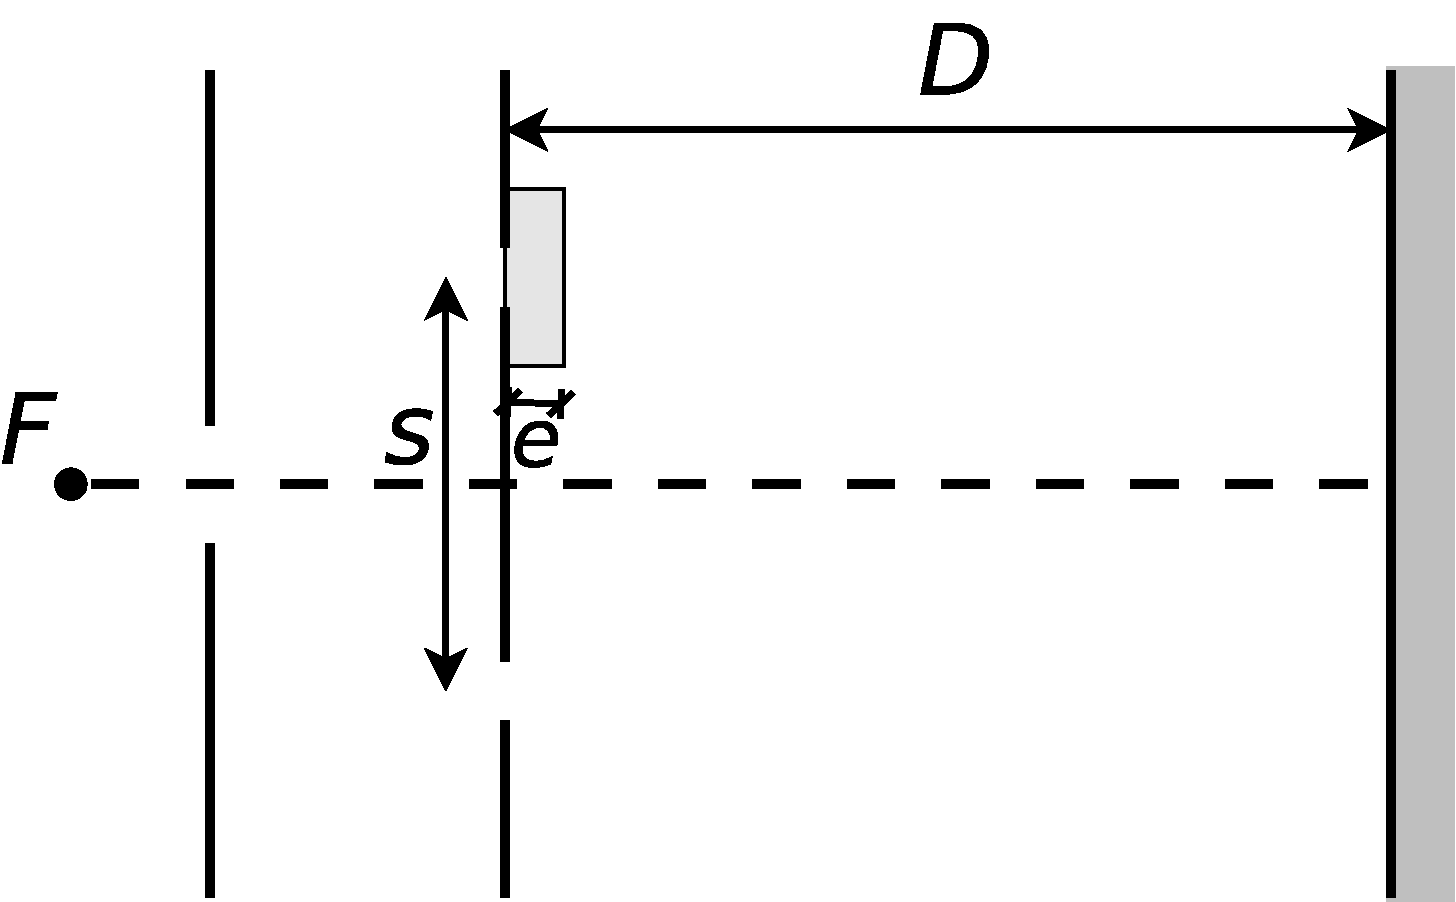
\includegraphics[width=\textwidth]{ej5-5}
\end{minipage}
Si se coloca detrás de una de las ranuras una lámina de vidrio de caras planas paralelas de un espesor $e = \SI{0.01}{\milli\metre}$ como muestra la figura, el patrón de franjas se deplazará.
Determine el sentido de tal desplazamiento y la fórmula que da la expresión de dicho desplazamiento.
Sabiendo que las franjas se han desplazado \SI{4.73}{\milli\metre}, calcule el valor del índice de refracción del vidrio.
¿Puede detectar dicho corrimiento con una fuente monocromática?
¿Y con una policromática?


\item ¿Cómo cambia el experimento de Young si la fuente luminosa no está simétricamente situada respecto de la ranura, o si, por algún motivo, las ondas que llegan a las mismas tienen un cierto desfasaje?
¿Cómo puede detectar dicho corrimiento?



%\item
%\begin{minipage}[t][5cm]{0.6\textwidth}
%(*) Se tiene el dispositivo para producir interferencia que indica la figura.
%La fuente puntual monocromática de longitud de onda $\lambda$ (linealmente polarizada en el eje $z$, con amplitud $E_{0}$), ilumina dos rendijas separadas por una distancia $a$.
%La fuente está centrada respecto de las rendijas y se encuentra a una distancia $L_{0}$ de las mismas.
%A la izquierda de las rendijas hay dos medios distintos; sobre el eje $x$ es $n_{1}$, y debajo del eje $x$ es $n_{2}$ ($n_{2}>n_{1}$); a la derecha de las rendijas el índice es $n_{1}$ solamente.
%A continuación de la rendija 2 se coloca una lámina polarizadora cuyo eje de transmisión forma un ángulo $\alpha$ con el eje $z$. 
%Datos: $a$, $n_{2}$, $n_{1}$, $E_{0}$, $L_{0}$, $L$.
%\end{minipage}
%\begin{minipage}[c][0cm][t]{0.35\textwidth}
%	\includegraphics[width=\textwidth]{ej5-7}
%\end{minipage}
%\begin{enumerate}
%	\item ¿Qué efecto produce en el patrón de interferencia la diferencia de medios?
%	Explique.
%	\item Halle el campo eléctrico que sale de la lámina polarizadora como función de $\alpha$; expréselo en las coordenadas $y-z$ (sólo el campo que sale de la ranura 2; no el total).
%	\item Halle la expresión de la intensidad en un punto $P$ de la pantalla, en función de los campos eléctricos a la salida de las rendijas 1 y 2.
%	Tenga en cuenta para esto la polarización de dichos campos.
%	\item Calcule el contraste $c=\frac{I_{m\acute{a}x}-I_{m\acute{\imath}n}}{I_{m\acute{a}x}\text{+}I_{m\acute{\imath}n}}$, en función del ángulo $\alpha$ y de $\theta$ (ángulo subtendido por P).
%	¿Existen ceros de intensidad para algún $\theta$?
%\end{enumerate}
